\documentclass[a4paper, twoside, 11pt]{article}
% It is needed to use this command for automatic compilation in VSCode
% !TEX program = lualatexmk

%DOCUMENT, PREAMBLE AND MACROS DESIGNED FOR LuaLaTeX%
\newcommand{\fbar}{\FloatBarrier}

\usepackage{amsmath} %matematic package%
\usepackage{amssymb} %for miscellaneous mathematical symbols, first usage was for tick symbol in math mode \checkmark%
\usepackage{textcomp} %for miscellaneous symbols%
%\usepackage{times} %times font%
\usepackage{graphicx} %enhanced support for craphics%
%\usepackage{mathptmx} %use Times as default text font, and provide maths support%
\usepackage{cmap} %mapování znaků - vyhledávání v pdf%
\usepackage[czech]{babel}%CZ%
\usepackage[utf8]{inputenc}%kódování%
\usepackage[T1]{fontenc}%kódování%
\usepackage{multirow}%Multirow table support
\usepackage{float}%Improves the interface for defining floating objects such as figures and tables%
\usepackage{wasysym} %for various glyphs, symbols%

\usepackage{setspace}%spacing% 
\onehalfspacing

\usepackage{hyperref}
\hypersetup{
    colorlinks=true, %pokud nechci definovat citecolor=black aby byly odkazy citací černé, tak dám colorlinks=false,%
    bookmarks=true,
    linkcolor=black,
    citecolor=black,
    urlcolor=black,
}

%when using LuaLaTex, defining Times Fonts from your system - it has to be named like this and inserted ttf file in the folder of your tex file%
\usepackage{fontspec}
\selectlanguage{czech}
\setmainfont[Ligatures=TeX,BoldFont={Times New Roman Bold}] {Times New Roman}
                                
\setsansfont[Ligatures=TeX,BoldFont={* Bold}]{Times New Roman}
                                      
\setmonofont{CourierPrime-Regular}
 
%\usepackage[italic]{mathastext} %for text in math environment, better looking times then



%for CITATIONS URL to work, it is not needed when you are not using URL label%
\usepackage{url}
\usepackage{csquotes}
\usepackage[style=iso-numeric, backend=biber, isbn=true, urldate=iso,seconds=true, date=terse, datezeros=true, language=czech]{biblatex}
\addbibresource{src/bib/zdroje.bib} % BIB resources to import
%\DeclareUrlCommand\url{\def\UrlLeft{<}\def\UrlRight{>} \urlstyle{tt}}



%\usepackage{biblatex}
%END for citations%

%changing bibliography font%
\renewcommand*{\bibfont}{\fontspec{Times New Roman}}

\usepackage{comment} %For comments%
\usepackage{pdfpages}%for pdf pages%
\usepackage{enumerate}%For lists%
\usepackage{enumitem}%For Custom Numbering Nested Lists%
\setlist[enumerate]{label*=\arabic*.} %setting Number. numbering in lists%
\usepackage{tikz} %For vector graphics%
\usepackage{circuitikz}%For schemes%
\usepackage{pgf} %Post script graphics for tikz%

%pouze funguje v PDFLaTeX%
%\usepackage{tgtermes}%na times font, jiný nefunguje s vyhledáváním a copy%

%
\usepackage{placeins}%% for \FloatBarrier command that blocks floating with htbp! go over \FloatBarrier
\usepackage{mathrsfs}%packagee for math symbols for Laplace, Z transform etc., usage \mathscr{Z}
\usepackage{upgreek}%for upgreek symbols, specified tau \uptau
\usepackage{physics}% for derivations \dd
%this works only when using PDFLaTeX%
\usepackage[list=true,listformat=simple]{subcaption}
\usepackage[figurename=Obr.,font=small,labelfont=it,textfont=it]{caption} %for renaming figures instead of renewcommand, small for 11pt default is 10pt as needed in word template
\usepackage[tablename=Tab.,font=small,labelfont=it,
            textfont=it]{caption} %for renaming tables instead of renewcommand
            

% List of abbreviations and symbols
% Original code author: Jakub Kučera

\usepackage[nonumberlist,nopostdot,section=subsection,numberedsection]{glossaries}
% section = subsection is for glossaries title to appear as a subsection, numberedsection adds the subsec number

\newglossary[slg]{symbolslist}{symbol}{ntn1}{Seznam symbolů}
\newglossary[slg]{abbreviationslist}{abbreviation}{ntn2}{Seznam zkratek}

\makeglossaries

% include files with definitions
% PZ definitions
\newglossaryentry{abbreviation:asm}{
                type=abbreviationslist,
                name={ASM},
                description={Asynchronní Motor}
}
\newglossaryentry{abbreviation:pmsynrelm}{
                type=abbreviationslist,
                name={PMSynRelM},
                description={Permanent Magnet Assisted Synchronous Reluctance Motor}
}
\newglossaryentry{abbreviation:synrelm}{
                type=abbreviationslist,
                name={SynRelM},
                description={Synchronous Reluctance Motor}
}
\newglossaryentry{abbreviation:pm}{
                type=abbreviationslist,
                name={PM},
                description={Permanent Magnets}
}
\newglossaryentry{abbreviation:pmsm}{
                type=abbreviationslist,
                name={PMSM},
                description={Permanent Magnet Synchronous Motor}
}
\newglossaryentry{abbreviation:dsp}{
                type=abbreviationslist,
                name={DSP},
                description={Digial Signal Processor}
}
\newglossaryentry{abbreviation:foc}{
                type=abbreviationslist,
                name={FOC},
                description={Field Oriented Control}
}
\newglossaryentry{abbreviation:dtc}{
                type=abbreviationslist,
                name={DTC},
                description={Direct Torque Control}
}
\newglossaryentry{abbreviation:mtpa}{
                type=abbreviationslist,
                name={MTPA},
                description={Maximum Torque Per Ampere}
}
\newglossaryentry{abbreviation:mtpv}{
                type=abbreviationslist,
                name={MTPV},
                description={Maximum Torque Per Voltage}
}
\newglossaryentry{abbreviation:emf}{
                type=abbreviationslist,
                name={EMF},
                description={Electromotive Force}
}
\newglossaryentry{abbreviation:upfc}{
                type=abbreviationslist,
                name={UPFC},
                description={Unity Power Factor Control}
}

\newglossaryentry{abbreviation:pwm}{
                type=abbreviationslist,
                name={PWM},
                description={Pulse Width Modulation}
}


\newglossaryentry{symbol:Pn}{
    type=symbolslist, % glossary
    name=$P_\text{n}$, % jméno v seznamu
    description={jmenovitý výkon}, %popis
    symbol = (W),
    sort=P % seředit podle
}

\newglossaryentry{symbol:Un}{
    type=symbolslist, % glossary
    name=$U_\text{n}$, % jméno v seznamu
    description={jmenovité sdružené napětí}, %popis
    symbol = (V),
    sort=U % seředit podle
}

\newglossaryentry{symbol:fn}{
    type=symbolslist, % glossary
    name=$f_\text{n}$, % jméno v seznamu
    description={jmenovitá napájecí frekvence}, %popis
    symbol = (Hz),
    sort=F% seředit podle
}

\newglossaryentry{symbol:cosphin}{
    type=symbolslist, % glossary
    name=$\cos(\varphi_\text{n})$, % jméno v seznamu
    description={jmenovitý účinník}, %popis
    symbol = (-),
    sort=P% seředit podle
}

\newglossaryentry{symbol:nn}{
    type=symbolslist, % glossary
    name=$n_\text{n}$, % jméno v seznamu
    description={jmenovité otáčky}, %popis
    symbol = (min$^{-1}$),
    sort=P% seředit podle
}


\newglossaryentry{symbol:In}{
    type=symbolslist, % glossary
    name=$I_\text{n}$, % jméno v seznamu
    description={jmenovitý fázový proud stroje}, %popis
    symbol = (A),
    sort=I % seředit podle
}

\newglossaryentry{symbol:u1}{
    type=symbolslist, % glossary
    name=$\underline{u_{1}^{k}}$, % jméno v seznamu
    description={prostorový vektor napětí statorového vinutí}, %popis
    symbol = (V),
    sort=U % seředit podle
}

\newglossaryentry{symbol:u2}{
    type=symbolslist, % glossary
    name=$\underline{u_{2}^{k}}$, % jméno v seznamu
    description={prostorový vektor napětí rotorového vinutí}, %popis
    symbol = (V),
    sort=U % seředit podle
}

\newglossaryentry{symbol:psi1}{
    type=symbolslist, % glossary
    name=$\underline{\psi_1^{k}}$, % jméno v seznamu
    description={prostorový vektor spřaženého magnetického toku statorového vinutí}, %popis
    symbol = (Wb),
    sort=P % seředit podle
}

\newglossaryentry{symbol:psi2}{
    type=symbolslist, % glossary
    name=$\underline{\psi_2^{k}}$, % jméno v seznamu
    description={prostorový vektor spřaženého magnetického toku rotorového vinutí}, %popis
    symbol = (Wb),
    sort=P % seředit podle
}

\newglossaryentry{symbol:r1}{
    type=symbolslist, % glossary
    name=$R_1$, % jméno v seznamu
    description={rezistivita statorového vinutí}, %popis
    symbol = ($\Omega$),
    sort=R % seředit podle
}

\newglossaryentry{symbol:r2}{
    type=symbolslist, % glossary
    name=$R_2$, % jméno v seznamu
    description={rezistivita rotorového vinutí}, %popis
    symbol = ($\Omega$),
    sort=R % seředit podle
}

\newglossaryentry{symbol:i1}{
    type=symbolslist, % glossary
    name=$\underline{i_1^{k}}$, % jméno v seznamu
    description={prostorový vektor proudu statorového vinutí}, %popis
    symbol = (A),
    sort=I % seředit podle
}

\newglossaryentry{symbol:i2}{
    type=symbolslist, % glossary
    name=$\underline{i_2^{k}}$, % jméno v seznamu
    description={prostorový vektor proudu rotorového vinutí}, %popis
    symbol = (A),
    sort=I % seředit podle
}

\newglossaryentry{symbol:omega}{
    type=symbolslist, % glossary
    name=$\omega$, % jméno v seznamu
    description={elektrická úhlová rychlost rotoru}, %popis
    symbol = (s$^{-1}$),
    sort=O % seředit podle
}

\newglossaryentry{symbol:omegas}{
    type=symbolslist, % glossary
    name=$\omega_\text{s}$, % jméno v seznamu
    description={skluzová elektrická úhlová rychlost}, %popis
    symbol = (s$^{-1}$),
    sort=O % seředit podle
}

\newglossaryentry{symbol:omegak}{
    type=symbolslist, % glossary
    name=$\omega_\text{k}$, % jméno v seznamu
    description={obecná elektrická úhlová rychlost}, %popis
    symbol = (s$^{-1}$),
    sort=O % seředit podle
}

\newglossaryentry{symbol:omegamech}{
    type=symbolslist, % glossary
    name=$\Omega$, % jméno v seznamu
    description={mechanická úhlová rychlost}, %popis
    symbol = (s$^{-1}$),
    sort=O % seředit podle
}

\newglossaryentry{symbol:omega1}{
    type=symbolslist, % glossary
    name=$\omega_1$, % jméno v seznamu
    description={elektrická úhlová rychlost točivého magnetického pole}, %popis
    symbol = (s$^{-1}$),
    sort=O % seředit podle
}

\newglossaryentry{symbol:l1}{
    type=symbolslist, % glossary
    name=$L_1$, % jméno v seznamu
    description={indukčnost statorového vinutí}, %popis
    symbol = (H),
    sort=L % seředit podle
}

\newglossaryentry{symbol:j}{
    type=symbolslist, % glossary
    name=$J$, % jméno v seznamu
    description={moment setrvačnosti}, %popis
    symbol = (kg$\cdot$m$^{2}$),
    sort=J % seředit podle
}

\newglossaryentry{symbol:l1sigma}{
    type=symbolslist, % glossary
    name=$L_{1\sigma}$, % jméno v seznamu
    description={rozyptylová indukčnost statorového vinutí}, %popis
    symbol = (H),
    sort=L % seředit podle
}

\newglossaryentry{symbol:l2sigma}{
    type=symbolslist, % glossary
    name=$L_{2\sigma}$, % jméno v seznamu
    description={rozyptylová indukčnost rotorového vinutí}, %popis
    symbol = (H),
    sort=L % seředit podle
}

\newglossaryentry{symbol:lm}{
    type=symbolslist, % glossary
    name=$L_\text{m}$, % jméno v seznamu
    description={magnetizační indukčnost}, %popis
    symbol = (H),
    sort=L % seředit podle
}

\newglossaryentry{symbol:l2}{
    type=symbolslist, % glossary
    name=$L_2$, % jméno v seznamu
    description={indukčnost rotorového vinutí}, %popis
    symbol = (H),
    sort=L % seředit podle
}

\newglossaryentry{symbol:pp}{
    type=symbolslist, % glossary
    name=$p_\text{p}$, % jméno v seznamu
    description={počet polpárů stroje}, %popis
    symbol = (-),
    sort=P % seředit podle
}

\newglossaryentry{symbol:m}{
    type=symbolslist, % glossary
    name=$M$, % jméno v seznamu
    description={vnitřní elektromechanický moment stroje}, %popis
    symbol = (Nm),
    sort=P % seředit podle
}

\newglossaryentry{symbol:mz}{
    type=symbolslist, % glossary
    name=$M$, % jméno v seznamu
    description={zátěžný moment}, %popis
    symbol = (Nm),
    sort=P % seředit podle
}

\newglossaryentry{symbol:slip}{
    type=symbolslist, % glossary
    name=$s$, % jméno v seznamu
    description={skluz}, %popis
    symbol = (-),
    sort=S % seředit podle
}

\newglossaryentry{symbol:u1ef}{
    type=symbolslist, % glossary
    name=$U_1$, % jméno v seznamu
    description={efektivní hodnota fázového napájecího napětí}, %popis
    symbol = (V),
    sort=U % seředit podle
}




\newglossarystyle{myStyleAbbreviations}{
\renewenvironment{theglossary}%
     {\begin{longtable}[l]{llp{\glsdescwidth}p{\glspagelistwidth}}}%
     {\end{longtable}}%
  \renewcommand*{\glossaryheader}{}%
  \renewcommand*{\glsgroupheading}[1]{}%
  \renewcommand{\glossentry}[2]{%
  \glsentryitem{##1} \glstarget{##1}{##2} &
    \textbf{\glossentryname{##1}} &
    \glossentrydesc{##1} &
    ##2\tabularnewline
  }%
  \renewcommand*{\glsgroupskip}{}%  Pokud chci seskupovat podle abeced: \renewcommand*{\glsgroupskip}{ & \\}
}


\newglossarystyle{myStyleSymbols}{
  \renewenvironment{theglossary}%
    {\begin{longtable}[l]{llp{\glsdescwidth}p{\glspagelistwidth}}}%
    {\end{longtable}}%
  \renewcommand*{\glossaryheader}{}%
  \renewcommand*{\glsgroupheading}[1]{}%
  \renewcommand{\glossentry}[2]{%
    \glsentryitem{##1} \glstarget{##1}{\glossentryname{##1}} &
    \glossentrysymbol{##1} &
    \glossentrydesc{##1} &
    ##2\tabularnewline
  }%
  \renewcommand{\subglossentry}[3]{%
     &
     \glssubentryitem{##2}%
     \glossentrysymbol{##2} &
     \glstarget{##2}{\strut}\glossentrydesc{##2} & ##3\tabularnewline
  }%
  \renewcommand*{\glsgroupskip}{%
   }% Pokud chci seskupovat podel abecedy  \ifglsnogroupskip\else & & &\tabularnewline\fi
}
\renewcommand{\glossarypreamble}{\vspace*{-\baselineskip}} % deleting line after glossaries title

            %this works with LuaLaTex and fontspec package%
 \DeclareCaptionFont{times}{\fontspec{Times New Roman Italic}}

%labelfont and textfont defined here only works with previous declarecaptionfont times and fontspec%
\captionsetup{labelfont=times, textfont=times, labelsep=space}%no separator in captions
%

%\bibliographystyle{czechiso} %czechiso.bst in folder is needed for this style to work, available at http://www.fit.vutbr.cz/~martinek/latex/czechiso.html%

%\hyperref[label]{text}% Help for targeting labels

\usepackage{chngcntr} %for numbered figures with sections
\usepackage{tocloft}%better TOC

%\usepackage{a4wide}%širší a4%
\usepackage[inner=3cm,outer=2cm,top=2.5cm,bottom=2.5cm,footskip=1cm]{geometry}%for propper margins
\usepackage{textcase}%for making text uppercase without caps \MakeTextUppercase
 
 
\usepackage{titlesec}%for spacing text after sections
\usepackage{parskip}[]%for working \parskip
\newcommand{\sectionbreak}{\clearpage}%maybe for SECTIONS on a new page

\usepackage[titletoc]{appendix}%For appendix - přílohy, titletoc is crucial
%\renewcommand{\appendixname}{Příloha}

\setlength{\parindent}{0.5cm}%setting indent of paragraph to 0.5cm
\setlength{\parskip}{0em}%setting parskip to 0 for \titleformat to work properly with parskip package

\usepackage{colortbl}%for colored cells
\usepackage{xcolor}%for colors
\definecolor{ctublue}{HTML}{0065BD}%defining ctu color
\definecolor{ctugreen}{HTML}{A2AD00}
\definecolor{ctured}{HTML}{C60C30}
\definecolor{ctuyellow}{HTML}{F0AB00}
\definecolor{ctugreenyblue}{HTML}{00B2A9}
\definecolor{ctulightblue}{HTML}{6AADE4}
\definecolor{ctuorange}{HTML}{E05206}
\definecolor{lightgray}{HTML}{D1D5DB}
\definecolor{codeblue}{HTML}{D9E2F3}


\titlespacing*{\section}{0em}{1em}{-\parskip}%spacing text after sections from titlesec package
\titlespacing*{\subsection}{0em}{1em}{-\parskip}%spacing text after sections from titlesec package
\titlespacing*{\subsubsection}{0em}{1em}{-\parskip}%spacing text after sections from titlesec package

%when you want sectin/sub/subsub to be black, delete \color{ctublue}
\titleformat{\section}{\color{ctublue}\fontspec{Times New Roman}\fontsize{15}{15}\bfseries}{\thesection}{2.1em}{}%defining title sizes by word template
\titleformat{\subsection}{\color{ctublue}\fontspec{Times New Roman}\fontsize{14}{14}\bfseries}{\thesubsection}{1.53em}{}%defining title sizes by word template
\titleformat{\subsubsection}{\color{ctublue}\fontspec{Times New Roman}\fontsize{13}{13}\bfseries}{\thesubsubsection}{1em}{}%defining title sizes by word template


\usepackage{ctable}%imports xtable with booktabs
\usepackage{multicol}

\usepackage{listings}%for code environments - \begin{lstlisting}


\definecolor{codegreen}{rgb}{0,0.6,0}
\definecolor{codegray}{rgb}{0.5,0.5,0.5}
\definecolor{codepurple}{rgb}{0.58,0,0.82}
\definecolor{backcolour}{rgb}{0.95,0.95,0.92}


% solving problems with ) literal to be coded in lstlisting as it should be
\makeatletter
\patchcmd{\lsthk@SelectCharTable}{)}{`}{}{} 
\makeatother 

\lstdefinestyle{zakopal}{
    backgroundcolor=\color{codeblue},   
    commentstyle=\color{codegray},
    keywordstyle=\color{ctured},
    numberstyle=\tiny\color{codegray},
    stringstyle=\color{ctuorange},
    basicstyle=\ttfamily\small,
    breakatwhitespace=false,         
    breaklines=true,                 
    captionpos=b,                    
    keepspaces=true,                 
    numbers=left,                    
    numbersep=5pt,                  
    showspaces=false,                
    showstringspaces=false,
    showtabs=false,                  
    tabsize=2
}
\lstset{style=zakopal}
\renewcommand{\lstlistingname}{Kód}% renaming Listing -> Kód 
\renewcommand{\lstlistlistingname}{List of codes}% renaming List of Listings -> Seznam kódů

\lstdefinelanguage{SCL}
{morekeywords={FUNCTION_BLOCK,BEGIN,NOT,END_FUNCTION_BLOCK,FUNCTION,VOID,VAR_INPUT,END_VAR,VAR_IN_OUT,IF,
THEN,END_IF,END_FUNCTION,BOOL,FALSE,TRUE},
sensitive=false,
morecomment=[l]{//},
morestring=[b]",
literate={;}{{\textcolor{ctuorange}{;}}}{1}
{:}{{\textcolor{ctuorange}{:}}}{1}
{)}{{\textcolor{ctuorange}{)}}}{1}
{(}{{\textcolor{ctuorange}{(}}}{1}
{=}{{\textcolor{ctuorange}{=}}}{1}
{,}{{\textcolor{ctuorange}{,}}}{1},} %basic SCL language for siemens defined%

\lstdefinelanguage{xdc}
{morekeywords={set_property, current_design, get_ports},
sensitive=false,
morecomment=[l]{\#}} %basic xdc file in Vivado syntax highlighting%

\lstdefinelanguage{xsct}
{morekeywords={xsct, hsi, open_hw_design, -createdts, -hw, -zocl, -platform-name, -overlay, -compile, -out, exit, -git-branch},
alsoletter={-},
sensitive=false,
morecomment=[l]{\#}} %xsct (Xilinx Software Command-Line Tools)%


\lstdefinelanguage{Text}
{morekeywords={},
alsoletter={-},
sensitive=false,
morecomment=[l]{//},
morecomment=[l]{\#}} %basic text%

\lstdefinelanguage{devicetree}
{morekeywords={chosen, bootargs, stdout-path, compatible, status},
alsoletter={-},
stringstyle=\color{ctuorange},
moredelim=[s][\color{ctuorange}]{"}{"},
sensitive=false,
morecomment=[l]{\#},
literate={\{}{{\textcolor{ctured}{\{}}}{1}
{\}}{{\textcolor{ctured}{\}}}}{1}
} %devicetree%

\lstdefinelanguage{json}
{morekeywords={},
upquote=true,
morestring=[b]",
stringstyle=\color{ctuorange},
moredelim=[s][\color{ctuorange}]{"}{"},
sensitive=false,
morecomment=[l]{\#},
literate=
     *{0}{{{\color{ctured}0}}}{1}
      {1}{{{\color{ctured}1}}}{1}
      {2}{{{\color{ctured}2}}}{1}
      {3}{{{\color{ctured}3}}}{1}
      {4}{{{\color{ctured}4}}}{1}
      {5}{{{\color{ctured}5}}}{1}
      {6}{{{\color{ctured}6}}}{1}
      {7}{{{\color{ctured}7}}}{1}
      {8}{{{\color{ctured}8}}}{1}
      {9}{{{\color{ctured}9}}}{1}
      {\{}{{{\color{ctured}{\{}}}}{1}
      {\}}{{{\color{ctured}{\}}}}}{1}
      {[}{{{\color{ctured}{[}}}}{1}
      {]}{{{\color{ctured}{]}}}}{1},
} %json%

\lstdefinelanguage{pseudocode}
{morekeywords={if, else, positive, negative, edge, end},
alsoletter={-},
stringstyle=\color{ctuorange},
moredelim=[s][\color{ctuorange}]{"}{"},
sensitive=false,
morecomment=[l]{\//},
literate={\{}{{\textcolor{ctured}{\{}}}{1}
{\}}{{\textcolor{ctured}{\}}}}{1}
{(}{{{\color{ctured}{(}}}}{1}
{)}{{{\color{ctured}{)}}}}{1}
} %devicetree%

%%change in previous commands 2.1 em , 1.53em and 1em to 1em to be easy indented not the same
\begin{document}
\fontspec{Times New Roman}

\counterwithin{figure}{section}%changing counter of figure, at each section the numbering resets
\counterwithin{table}{section}%changing counter of table, at each section the numbering resets
\counterwithin{equation}{section}%changing counter of equation, at each section the numbering resets

\counterwithin{lstlisting}{section}%counter of lstlist - codes, reseting at each section%


\renewcommand{\thefigure}{\thesection~-~\arabic{figure}}%defining style of countering
\renewcommand{\thetable}{\thesection~-~\arabic{table}}
\renewcommand{\theequation}{\thesection~-~\arabic{equation}}
\renewcommand{\thelstlisting}{\thesection~-~\arabic{lstlisting}}%delfining style for lstlisting codes, needs to be after begin document as previous renewcommand%

\renewcommand*{\cftsecdotsep}{1}  % use dots in the section entries and their step
\renewcommand*{\cftsubsecdotsep}{1}
\renewcommand*{\cftsubsubsecdotsep}{1}
\renewcommand*{\cftsecnumwidth}{4em} % increase space for Roman numerals
\renewcommand*{\cftsubsecnumwidth}{4em} %numbering width
\renewcommand*{\cftsubsubsecnumwidth}{4em} %numbering width
\renewcommand*{\cftsubsubsecindent}{0em}%no indent for subsubsection
\renewcommand*{\cftsubsecindent}{0em}%no indent for subsection
\renewcommand*{\cftsecindent}{0em}%no indent for subsection



\renewcommand*{\cftfigdotsep}{1}  % use dots in the figure entries and their step
\renewcommand*{\cftfignumwidth}{4em}
\renewcommand*{\cftfigindent}{0em}

\renewcommand*{\cfttabdotsep}{1}  % use dots in the figure entries and their step
\renewcommand*{\cfttabnumwidth}{4em}
\renewcommand*{\cfttabindent}{0em}

\renewcommand{\cftsecfont}{\fontspec{Times New Roman}\large \bfseries}
\renewcommand{\cftsubsecfont}{\fontspec{Times New Roman}}
\renewcommand{\cftsubsubsecfont}{\fontspec{Times New Roman}}

\renewcommand{\cftfigfont}{\fontspec{Times New Roman}}
\renewcommand{\cfttabfont}{\fontspec{Times New Roman}}

\renewcommand*\contentsname{\textcolor{ctublue}{\MakeTextUppercase{\fontspec{Times New Roman}Obsah}}}
\renewcommand{\listtablename}{{\fontspec{Times New Roman}\textcolor{ctublue}{\MakeTextUppercase{{Seznam tabulek}}}}}
\renewcommand{\listfigurename}{{\fontspec{Times New Roman}\textcolor{ctublue}{\MakeTextUppercase{{Seznam obrázků}}}}}



%\renewcommand{\thefigure}{\arabic{section}.\arabic{figure}}%changing figure name to be section.subsection. but do no reset
\setcounter{figure}{0}

\begin{titlepage}
	\begin{center}

\begin{figure}[H]
	\begin{center}
		
\includegraphics[scale=1]{src/misc/symbol_cvut_konturova_verze.pdf}
	\end{center}
\end{figure}
	{\Large{\textbf{ČESKÉ VYSOKÉ UČENÍ TECHNICKÉ V~PRAZE}}}\\
	{\textbf{Fakulta elektrotechnická}}\\
	{\textbf{Katedra elektrických pohonů a trakce}}
	
	\vspace{3cm}
	
	
	{\Large\textbf{Tvorba modelu asynchronního motoru}}
	
	\vspace{1cm}
	
	%{\Large\textbf{Possibilities of Using SoC Platform Processors for Controlling Electric Drives}}
	
	%\vspace{2cm}
	
	1. úloha předmětu XP14DES\\
	
	\end{center}
	
	\vspace{3cm}
	
	%\noindent Studijní program: Elektrotechnika, Energetika a Management\\
	%\noindent Studijní obor: Elektrické pohony
	
	\vspace{0.5cm}
	%\noindent Vedoucí práce: doc. Ing. Jan Bauer, Ph.D.
	
	\vfill
	
\begin{center}

	\large{\textbf{Petr Zakopal}}\\
	\large{\textbf{Praha 2023}}
	\end{center}
\end{titlepage}


\newpage
%\pagenumbering{arabic} to arabic page numbering
\pagenumbering{gobble} %disabling page numbering

\newpage


%%ZADÁNÍ PRÁCE
%verze pro TISK - jen s NEW PAGE


%ONLINE VERZE - se zadáním BEZ PODPISŮ
% online verze - odkomentovat následující dva řádky
%\null\newpage
%\includepdf[]{src/docs/zadani_bez_podpisu.pdf}

%\newpage
%\cleardoublepage
\null\newpage

\pagenumbering{Roman}
\setcounter{page}{2}%%3 NUTNO řešit dle zadání etc.

% \noindent \textcolor{ctublue}{{\Large{\textbf{\MakeTextUppercase{Prohlášení}}}}}\\
% 			Prohlašuji, že jsem předloženou práci vypracoval samostatně a že jsem uvedl veškeré použité informační zdroje v~souladu s~Metodickým pokynem o~dodržování etických principů při přípravě vysokoškolských závěrečných prací.\\
% 		\vspace{1.5cm}
		
	

% 	\noindent	V~Praze dne \rule{3.5cm}{0.4pt} \hspace{6.6cm}  \rule{4cm}{0.4pt}
	
% 	\hspace{12.65cm}Petr Zakopal


% 		\vspace{14cm}
		
% 	\noindent	\textcolor{ctublue}{{\Large{\textbf{\MakeTextUppercase{Poděkování}}}}}\\
% 	Tímto bych rád poděkoval vedoucímu této práce doc. Ing. Janu Bauerovi, Ph.D. za skvělé vedení práce a cenné rady při jejím vytváření. Dále bych rád poděkoval všem, kteří mě v~mém dosavadním studiu podporovali.
		


%%ABSTRAKT%%

% \newpage
% %\addcontentsline{toc}{section}{3\quad Abstrakt a klíčová slova}%Added citations to TOC%
% %\begin{comment}
% \begin{minipage}[t]{7.37cm}
% 		%\raggedright
% 	\textcolor{ctublue}{\Large{\textbf{\MakeTextUppercase{Abstrakt}}}}\\
	
% \end{minipage}%
% \hfill% --- important, otherwise it wont be so nice
% \begin{minipage}[t]{7.37cm}
% 		\textcolor{ctublue}{\Large{\textbf{\MakeTextUppercase{Abstract}}}}\\
		
% \end{minipage}
% %\end{comment}
% 	%\textcolor{ctublue}{\Large{\textbf{\MakeTextUppercase{Abstrakt}}}}\\

% 	%\textcolor{ctublue}{\Large{\textbf{\MakeTextUppercase{Abstract}}}}\\

% \newpage
\tableofcontents
\newpage%
\flushbottom %vyčištění stránky
\newpage
\vspace{0pt}
\listoffigures %seznam obrázků
\flushbottom %vyčištění stránky
\newpage
\listoftables
\flushbottom
\newpage


\pagenumbering{arabic} %to arabic page numbering - enabling page numbering after gobble which disabled page numbering
\pagenumbering{gobble}
\null\newpage
% \null\newpage %PŘI VERZI ONLINE
\setcounter{page}{1}
\pagenumbering{arabic}
\fontspec{Times New Roman}

\section{Rovnice asynchronního motoru - využívané pro řízení}
Rovnice pro \gls{abbreviation:asm} je možné odvodit při uvažování následujících zjednodušení:

\begin{itemize}
    \item tloušťka vzduchové mezery je po celém obvodu mezi rotorem a statorem konstatní,
    \item statorová a rotorová vinutí jsou rozložena podél obvodu vzduchové mezery sinusově, vinutí jednotlivých fází jsou proti vůči sobě natočeny o~120 °,
    \item ztráty v~železe jsou zanedbány,
    \item není uvažováno sycení magnetického obvodu,
    \item aktivní železo stroje má nekonečnou relativní permeabilitu,
    \item statorová a rotorová vinutí jsou souměrná, tj. činné odpory, indukčnosti a vzájemné indukčnosti jednotlivých fází jsou identické.
\end{itemize}

Při uvažování uvedených zjednodušení je poté možné vyjádřit rovnice matematického modelu stroje v obecném souřadnicovém systému $k$.

 \begin{equation}
     \underline{u_{1}^{k}} = R_1 \underline{i_1^{k}} + \frac{\dd{\underline{\psi_1^{k}}}}{\dd{t}} + \text{j} \omega_k \underline{\psi_1^{k}},
    \end{equation}

    \begin{equation}
        \underline{u_{2}^{k}} = R_2 \underline{i_2^{k}} + \frac{\dd{\underline{\psi_2^{k}}}}{\dd{t}} + \text{j} (\omega_k - \omega) \underline{\psi_2^{k}},
    \end{equation}

    \begin{equation}
        \underline{\psi_1^{k}} = L_1 \underline{i_1^{k}} + L_\text{m} \underline{i_2^{k}},
    \end{equation}

    \begin{equation}
        \underline{\psi_2^{k}} = L_2 \underline{i_2^{k}} + L_\text{m} \underline{i_1^{k}}.
    \end{equation}

    Kde $k$ v horním indexu značí obecný souřadnicový systém, \gls{symbol:u1} (V) značí prostorový vektor napětí statorového vinutí, \gls{symbol:u2} (V) prostorový vektor napětí rotorového vinutí, \gls{symbol:psi1} (Wb) prostorový vektor spřaženého magentického toku statorového vinutí, \gls{symbol:psi2} (Wb) prostorový vektor spřaženého magnetického toku rotorového vinutí, \gls{symbol:r1} ($\Omega$) rezistivita statorového vinutí, \gls{symbol:r2} ($\Omega$) rezistivita rotorového vinutí, \gls{symbol:i1} (A) prostorový vektor proudu statorového vinutí, \gls{symbol:i2} (A) prostorový vektor proudu rotorového vinutí, \gls{symbol:omega} (s$^{-1}$) elektrická úhlová rychlost rotoru, \gls{symbol:omegas} (s$^{-1}$) skluzová rychlost, \gls{symbol:omegak} (s$^{-1}$) obecná úhlová rychlost, \gls{symbol:l1} (H) indukčnost statorového vinutí, \gls{symbol:l2} (H) indukčnost rotorového vinutí.\par

    V tomto textu jsou rovnice uvedeny obecně. Ovšem velmi často bývá uvažován \gls{abbreviation:asm} s kotvou nakrátko. Pro jeho model je možné uvažovat $\underline{u_{2k}} = 0$.\par


    \subsection{Rovnice pro soustavu spojenou se statorovým vinutím}
    V případě uvažování souřadné soustavy spojené se statorovým vinutím stroje, je možné upravit a zjedodušit rovnice popisující systém dle následujících vztahů. Souřadnicový systém spojený se statorovým vinutím se v literatuře často označuje jako systém $\alpha\beta$. Pro obecnou otáčivou rychlost \gls{symbol:omegak} soustavy platí $\omega_k$ = 0. Rovnice popisující model v uvedeném souřadnicovém systému jsou označeny \ref{eq:u1alphabeta} až \ref{eq:psi2alphabeta}.

 \begin{equation}\label{eq:u1alphabeta}
     \underline{u_{1}^{\alpha\beta}} = R_1 \underline{i_1^{\alpha\beta}} + \frac{\dd{\underline{\psi_1^{\lpha\beta}}}}{\dd{t}},
    \end{equation}

    \begin{equation}
        \underline{u_{2}^{\alpha\beta}} = R_2 \underline{i_2^{\alpha\beta}} + \frac{\dd{\underline{\psi_2^{\alpha\beta}}}}{\dd{t}} - \text{j} \omega \underline{\psi_2^{\alpha\beta}},
    \end{equation}

    \begin{equation}
        \underline{\psi_1^{\alpha\beta}} = L_1 \underline{i_1^{\alpha\beta}} + L_\text{m} \underline{i_2^{\alpha\beta}},
    \end{equation}

    \begin{equation}\label{eq:psi2alphabeta}
        \underline{\psi_2^{\alpha\beta}} = L_2 \underline{i_2^{\alpha\beta}} + L_\text{m} \underline{i_1^{\alpha\beta}}.
    \end{equation}
    \subsection{Rovnice pro soustavu spojenou s rotorovým vinutím}
    V případě uvažování modelu \gls{abbreviation:asm} v souřadnicovém systému spojeném s rotorovým vinutím platí pro obecnou otáčivou rychlost obecných rovnic $\omega_k = \omega$, kde $\omega$ (s$^{-1}$) je elektrická úhlová rychlost otáčení rotoru (rotorového vinutí). Souřadnicový systém je možné označit jako $kl$. Rovnice popisující model v uvedeném souřadnicovém systému jsou označeny \ref{eq:u1kl} až \ref{eq:psi2kl}.\par

 \begin{equation}\label{eq:u1kl}
     \underline{u_{1}^{kl}} = R_1 \underline{i_1^{kl}} + \frac{\dd{\underline{\psi_1^{kl}}}}{\dd{t}} + \text{j} \omega \underline{\psi_1^{k}},
    \end{equation}

    \begin{equation}
        \underline{u_{2}^{kl}} = R_2 \underline{i_2^{kl}} + \frac{\dd{\underline{\psi_2^{kl}}}}{\dd{t}},
    \end{equation}

    \begin{equation}
        \underline{\psi_1^{kl}} = L_1 \underline{i_1^{kl}} + L_\text{m} \underline{i_2^{kl}},
    \end{equation}

    \begin{equation}\label{eq:psi2kl}
        \underline{\psi_2^{kl}} = L_2 \underline{i_2^{kl}} + L_\text{m} \underline{i_1^{kl}}.
    \end{equation}

    \subsection{Rovnice pro soustavu spojenou s točivým magnetickým polem}
    Souřadnicový systém spojený s točivým magnetickým polem je velmi často označován jako systém $dq$. Pro obecnou úhlovou rychlost platí $\omega_k = \omega_1$, kde \gls{symbol:omega1} (s$^{-1}$) je elektrická úhlová rychlost točivého magnetického pole statoru, resp. rotoru.  Rovnice popisující model v uvedeném souřadnicovém systému jsou označeny \ref{eq:u1dq} až \ref{eq:psi2dq}.\par

 \begin{equation}\label{eq:u1dq}
     \underline{u_{1}^{dq}} = R_1 \underline{i_1^{dq}} + \frac{\dd{\underline{\psi_1^{dq}}}}{\dd{t}} + \text{j} \omega_1 \underline{\psi_1^{dq}},
    \end{equation}

    \begin{equation}
        \underline{u_{2}^{dq}} = R_2 \underline{i_2^{dq}} + \frac{\dd{\underline{\psi_2^{dq}}}}{\dd{t}} + \text{j} (\omega_1 - \omega) \underline{\psi_2^{dq}},
    \end{equation}

    \begin{equation}
        \underline{\psi_1^{dq}} = L_1 \underline{i_1^{dq}} + L_\text{m} \underline{i_2^{dq}},
    \end{equation}

    \begin{equation}\label{eq:psi2dq}
        \underline{\psi_2^{dq}} = L_2 \underline{i_2^{dq}} + L_\text{m} \underline{i_1^{dq}}.
    \end{equation}

    Velmi často se rozdíl $\omega_1 - \omega$ označuje jako skluzuvá rychlost $\omega_\text{s}$ (s$^{-1}$).
\section{Rovnice asynchronního motoru - využívané pro modelování}
Představené rovnice jsou např. vhodné pro modelování stroje při využívání \gls{abbreviation:foc}. Existuje mnoho dalších vyjádření představených rovnic podle toho, co je od modelu očekáváno a jaké veličiny je snadné měřit a které dopočítávat pomocí modelu.\par
Velmi často se v literatuře objevuje stavový popis modelu stroje s různými stavovými veličinami. V případě již zmiňovaného \gls{abbreviation:foc} se jako stavových proměnných využívá prostorových vektorů proudu statorového vinutí $\underline{i_1}$ např. v souřadnicové soustavě spojené se statorovým vinutím ($\underline{i_1^{\alpha\beta}}$) a spřažených magnetických toků rotorového vinutí \gls{symbol:psi2} (opět např. vyjádřených v systému spojeném se statorovým vinutím $\psi_2^{\alpha\beta})$.\par
V \cite{popescu-induction-motor-modelling-for-vector-control-purposes} jsou uvedeny stavové popisy pro uvedený systém v poměrných jednotkách. Pokud poměrné jednotky nejsou využívány, je možné modely převést na zjednodušené popisy v absolutních jednotkách, jako je tomu např. v \cite{lipcak-bauer-ept-moodle}.\par
Model implementovaný v prostředí MATLAB je převzat ze stavového popisu uvedeném v \cite{lipcak-bauer-ept-moodle}. Tento stavový popis je uveden v rovnici \ref{eq:state-equations-asm-model-lipcak}. 

\begin{equation}\label{eq:state-equations-asm-model-lipcak}
    \frac{\dd{}}{\dd{t}}
    \begin{bmatrix}
        i_{1\alpha}\\
        i_{1\beta}\\
        \psi_{2\alpha}\\
        \psi_{2\beta}
    \end{bmatrix}
    =
    \begin{bmatrix}
        -\frac{R_2 L_\text{m}^{2} + L_2^2 R_1}{\sigma L_1 L_2^2} & 0 & \frac{L_\text{m} R_2}{\sigma L_1 L_2^2} & \frac{L_\text{m}}{\sigma L_1 L_2} \omega\\
        0 & - \frac{R_2 L_\text{m}^2 + L_2^2 R_1}{\sigma L_1 L_2^2} & - \frac{L_\text{m}}{\sigma L_1 L_2} \omega & \frac{L_\text{m} R_2}{\sigma L_1 L_2^2}\\
        \frac{L_\text{m} R_2}{L_2} & 0 & - \frac{R_2}{L_2} & -\omega\\
        0 & \frac{L_\text{m} R_2}{L_2} & \omega -\frac{R_2}{L_2}
    \end{bmatrix}
    \begin{bmatrix}
        i_{1\alpha}\\
        i_{1\beta}\\
        \psi_{2\alpha}\\
        \psi_{2\beta}
    \end{bmatrix}
    +
    \begin{bmatrix}
        \frac{1}{\sigma L_1} & 0\\
        0 & \frac{1}{\sigma L_1}\\
        0 & 0\\
        0 & 0
    \end{bmatrix}
    \begin{bmatrix}
        u_{1\alpha}\\
        u_{2\beta}
    \end{bmatrix}.
\end{equation}

Stavový popis je vhodné doplnit o~další rovnice, jež budou v~simulaci využity.

\begin{equation}
    M = \frac{3}{2} p_\text{p} \frac{L_\text{m}}{L_2} (\psi_{2\alpha} i_{1\beta} - \psi_{2\beta} i_{1\alpha}),
\end{equation}

\begin{equation}
    M - M_\text{z} = J \frac{\dd{\Omega}}{\dd{t}},
\end{equation}
\begin{equation}
    \omega = p_\text{p} \Omega,
\end{equation}
kde $\sigma = 1 - L_\text{m}^{2}/(L_1 L_2)$ (-) je tzv. rozptyl, $i_{1\alpha}$ (A) a $i_{1\beta}$ (A) jsou složky vektoru statorového proudu $\underline{i_1}$ (A), $\psi_{2\alpha}$ (Wb) a $\psi_{2\beta}$ (Wb) jsou složky vektoru rotorového magnetického toku $\underline{\psi_2}$ (Wb), $u_{1\alpha}$ (V) a $u_{1\beta}$ (V) jsou složky statorového napětí $\underline{u_1}$ (V), \gls{symbol:pp} (-) je počet polpárů stroje, \gls{symbol:omega} (s$^{-1}$) je elektrická úhlová rychlost hřídele, \gls{symbol:omegamech} (s$^{-1}$) je mechanická úhlová rychlost hřídele, \gls{symbol:m} je vnitřní elektromechanický moment stroje a \gls{symbol:mz} (Nm) je moment zátěžný.\par

Velmi často dochází k porovnání dynamické a statické charakteristiky elektromagnetického momentu stroje. Závislost hnacího momentu na skluzu, resp. úhlové rychlosti točivého magnetického pole je uvedena v rovnici \ref{eq:elektromagneticky-moment-pro-statickou-charakteristiku}.

 \begin{equation}\label{eq:elektromagneticky-moment-pro-statickou-charakteristiku}
            M_\text{h} = \frac{3 p_\text{p} U_\text{1}^{2}}{s \omega_1} \frac{1}{(R_1 + \frac{R_2}{s})^{2} + (\omega_1 L_{1\sigma} + s~\omega_1 L_{2\sigma})^{2}},
        \end{equation}
        kde \gls{symbol:slip} (-) je skluz, \gls{symbol:omega1} (s$^{-1}$) je úhlová rychlost točivého magnetického pole, \gls{symbol:u1ef} (V) efektivní hodnota fázového napájecího napětí, v~tomto případě je využito jmenovitého napětí motoru $380/\sqrt{3}$ V.


\section{Simulované závislosti elektromagnetického momentu na otáčkách stroje}
    Díky matematickému modelu stroje, vytvořeném v prostředí MATLAB Simulink, je možné vynést charakteristik veličin, které jsou v reálném prostředí neměřitelné. V případě této práce je vynesena závislost elektromagnetického (hnacího) momentu stroje na otáčkách stroje při změně vybraných veličin.\par
    Vybrané veličiny jsou následující:
    \begin{itemize}
            velikost rezistivity rotorového vinutí/kotvy stroje $R_2$ (např. při změně oteplení stroje),
            velikost rezistivity statorového vinutí $R_1$ (např. při změně oteplení stroje),
            velikost magnetizační indukčnosti stroje $L_\text{m}$,
            velikost rozptylové indukčnosti statorového vinutí $L_{1\sigma}$,
            velikost rozptylové indukčnosti rotorového viutí $L_{2\sigma}$.
    \end{itemize}

    \noindent Model stoje byl vytvořen na základě reálného stroje, umístěného v laboratoři H-26. Vinutí stroje je spojeno do hvězdy.\par

    \begin{minipage}[t]{0.47\textwidth}
        \vspace{\baselineskip}
        \begin{table}[H]
            \caption{Štítkové údaje stroje.}
            \centering
                \begin{tabular}{!{\vrule width 2pt} c | c !{\vrule width 2pt}}\noalign{\hrule height 2pt}
                    $P_\text{n}$ & 12 kW \\ \hline
                    $U_\text{n}$ & 380 V~\\ \hline
                    $I_\text{n}$ & 22 A\\ \hline
                    $n_\text{n}$ & 1460 min$^{-1}$ \\ \hline
                    $f_\text{n}$ & 50 Hz \\ \hline
                    $\cos(\varphi_\text{n})$ &  0.8 \\ \hline
                    $p_\text{p}$ & 2 \\ \noalign{\hrule height 2pt}
                \end{tabular}     
            \label{tab:stitkove-udaje}
        \end{table}
        \end{minipage}% --- important, otherwise it wont be so nice
        \hfill
        \begin{minipage}[t]{0.47\textwidth}
            \vspace{0pt}
            \begin{table}[H]
                \caption{Změřené parametry stroje.}
                \centering
                    \begin{tabular}{!{\vrule width 2pt} c | c !{\vrule width 2pt}}\noalign{\hrule height 2pt}
                        $R_\text{1}$ & 370 m$\Omega$ \\ \hline
                        $R_\text{2}$ & 225 m$\Omega$ \\ \hline
                        $L_{1\sigma}$ & 2,27 mH \\ \hline
                        $L_{2\sigma}$ & 2,27 mH \\ \hline
                        $L_\text{m}$ & 82,5 mH \\ \hline
                        $L_{1}$ & 84,77 mH \\ \hline
                        $L_{2}$ & 84,77 mH \\ \hline $J$ & 0,4 kg$\cdot$m$^{2}$ \\ \noalign{\hrule height 2pt}
                    \end{tabular}     
                \label{tab:zmerene-parametry-stroje}
            \end{table}
        \end{minipage}

        \vspace*{1cm}
Kde \gls{symbol:Pn} (W) je jmenovitý výkon stroje, \gls{symbol:In} (A) je jmenovitý fázový proud stroje (efektivní hodnota), \gls{symbol:Un} (V) je jmenovité sdružené napájací napětí stroje, \gls{symbol:fn} (Hz) je jmenovitá napájecí frekvence stroje, \gls{symbol:cosphin}~$(-)$ je jmenovitý účinník stroje, \gls{symbol:nn} (min$^{-1}$) jsou jmenovité otáčky stroje, \gls{symbol:pp} $(-)$ je počet polpárů stroje, \gls{symbol:r1}~($\Omega$), resp. \gls{symbol:r2} ($\Omega$) je statorový, resp. rotorový odpor, \gls{symbol:l1sigma} (H), resp. \gls{symbol:l2sigma} (H) je statorová, resp. rotorová rozptylová  indukčnost stroje, \gls{symbol:lm} (H) je magnetizační indukčnost stroje, \gls{symbol:l1} (H), resp. \gls{symbol:l2} (H) je statorová, resp. rotorová indukčnost, \gls{symbol:j} (kg$\cdot$m$^{2}$) je moment setrvačnosti hřídele.\par

\newpage
    \subsection{Změna rezistivity rotorového vinutí}
        \begin{figure}[htbp!]
            \centering
            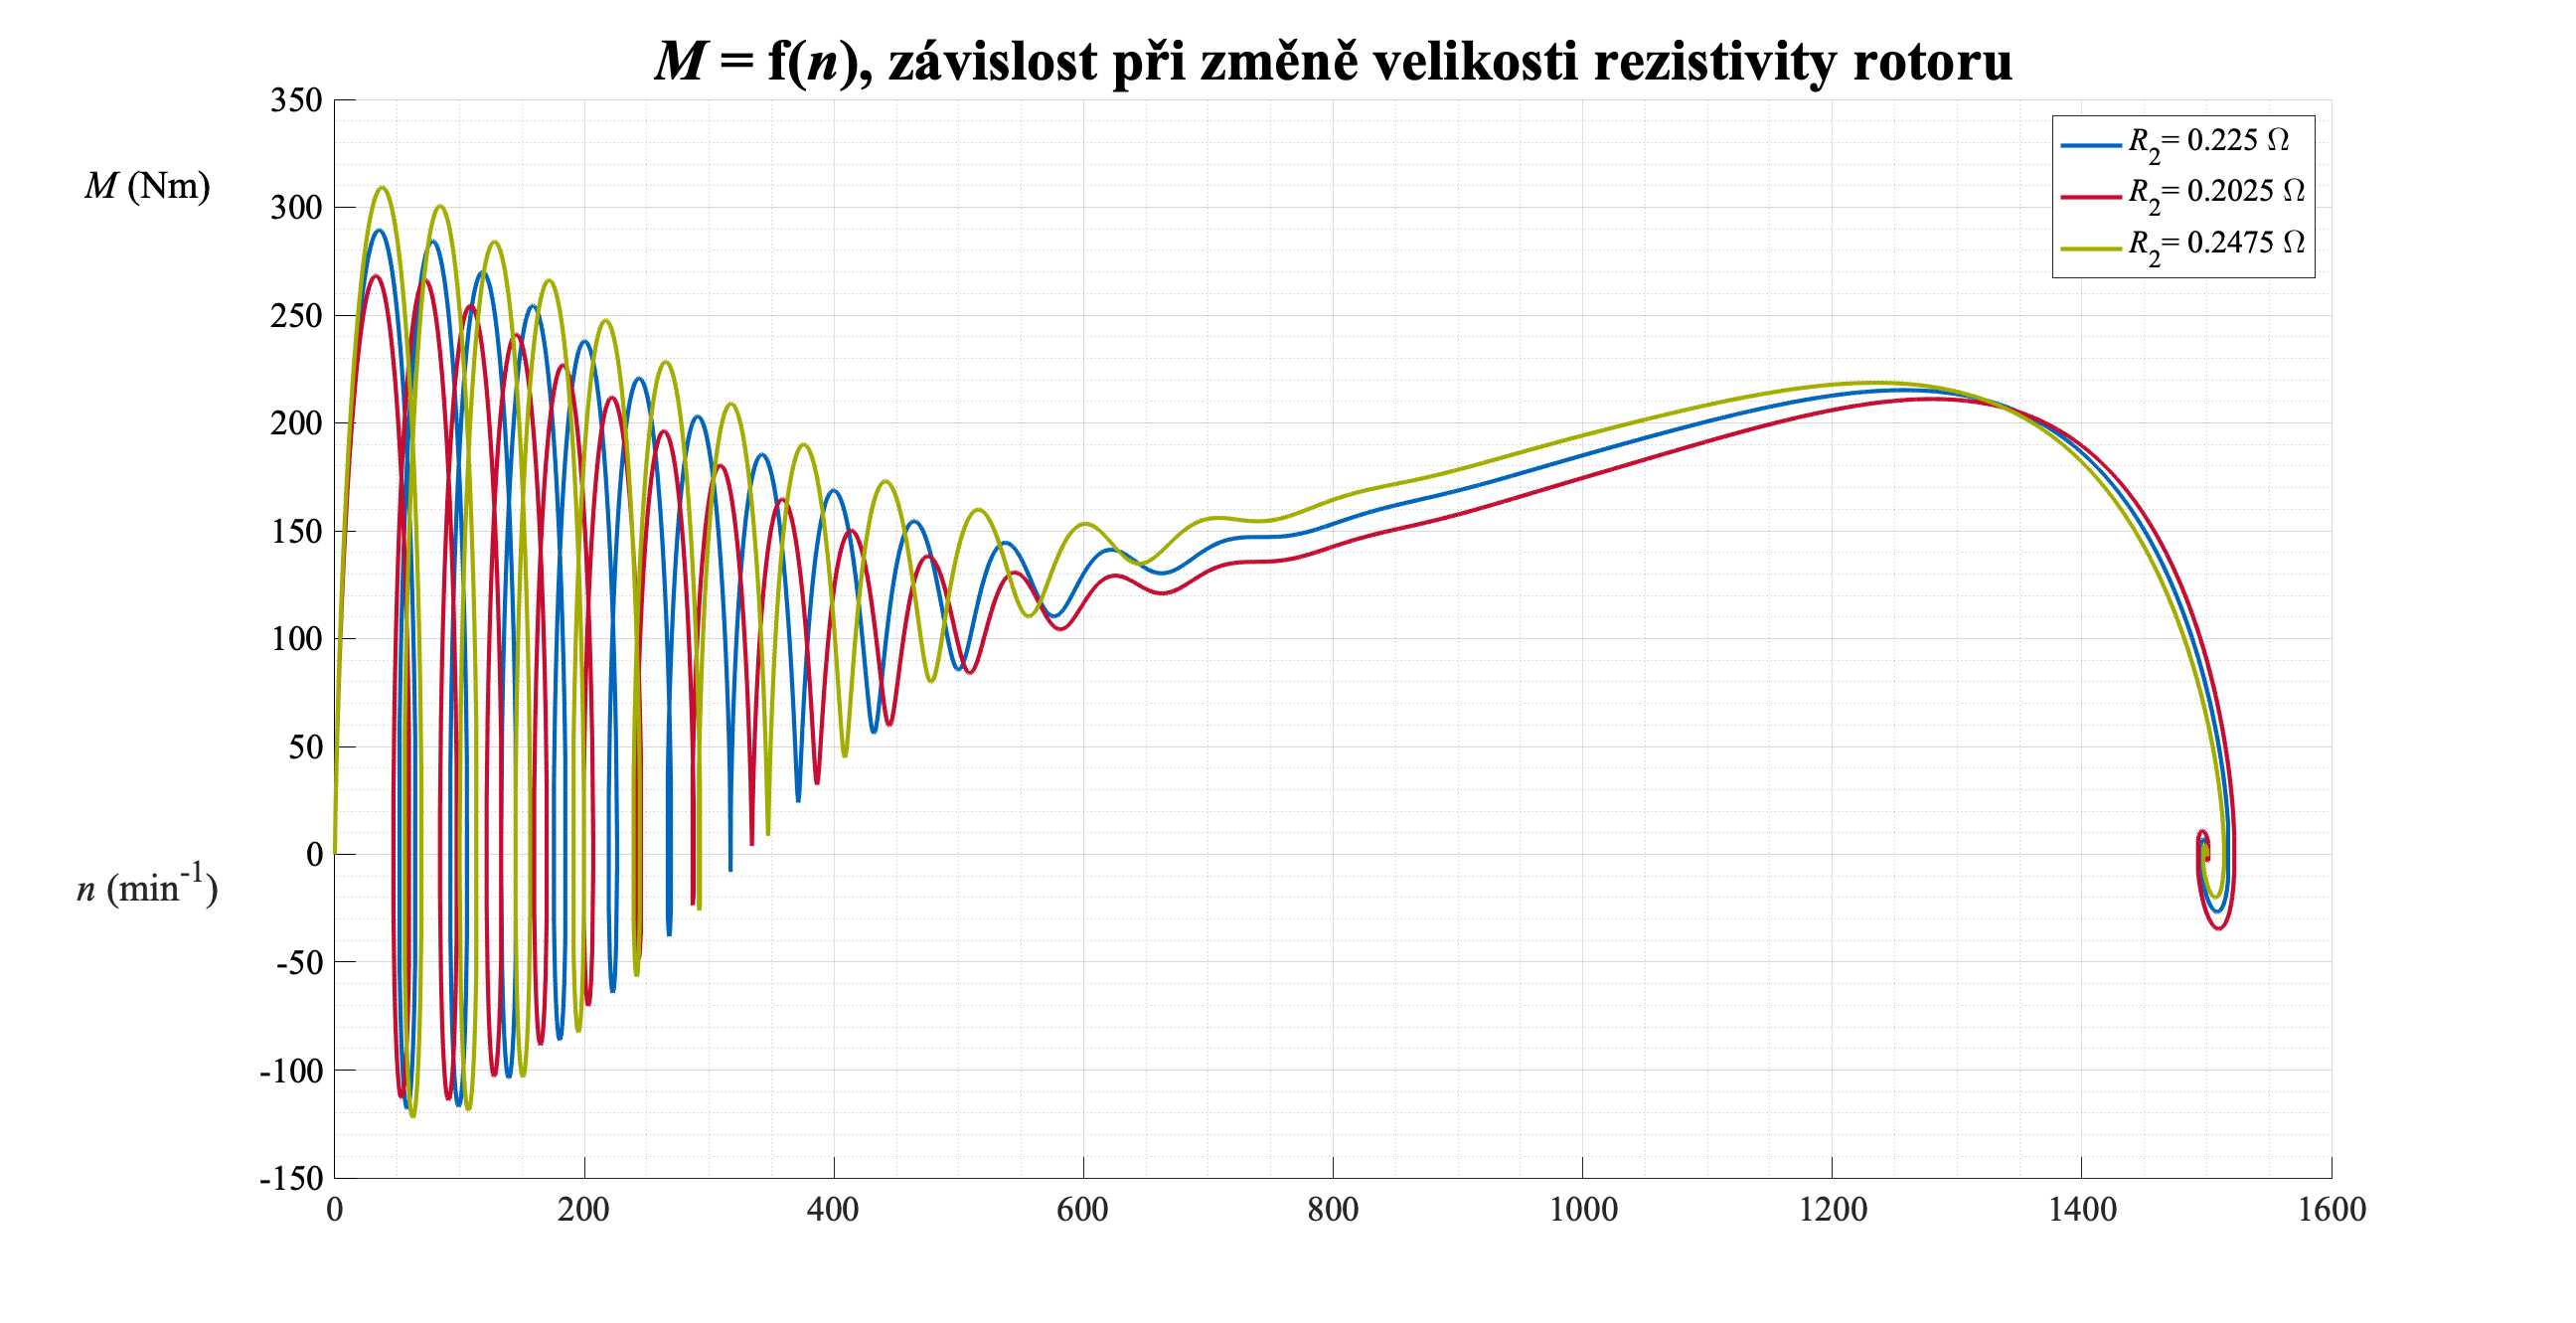
\includegraphics[width=1\textwidth]{src/png/mh_dyn_nGraphR2.png}
            \caption{Závislost elektromagnetického hnacího momentu \gls{symbol:m} na otáčkách stroje, vynesená při změně rezistivity rotorového viutí o $\pm 10 \%$.}
            \label{fig:mh_dyn_nGraphR2}
        \end{figure}

    \fbar
    \subsection{Změna rezistivity statorového vinutí}
        \begin{figure}[htbp!]
            \centering
            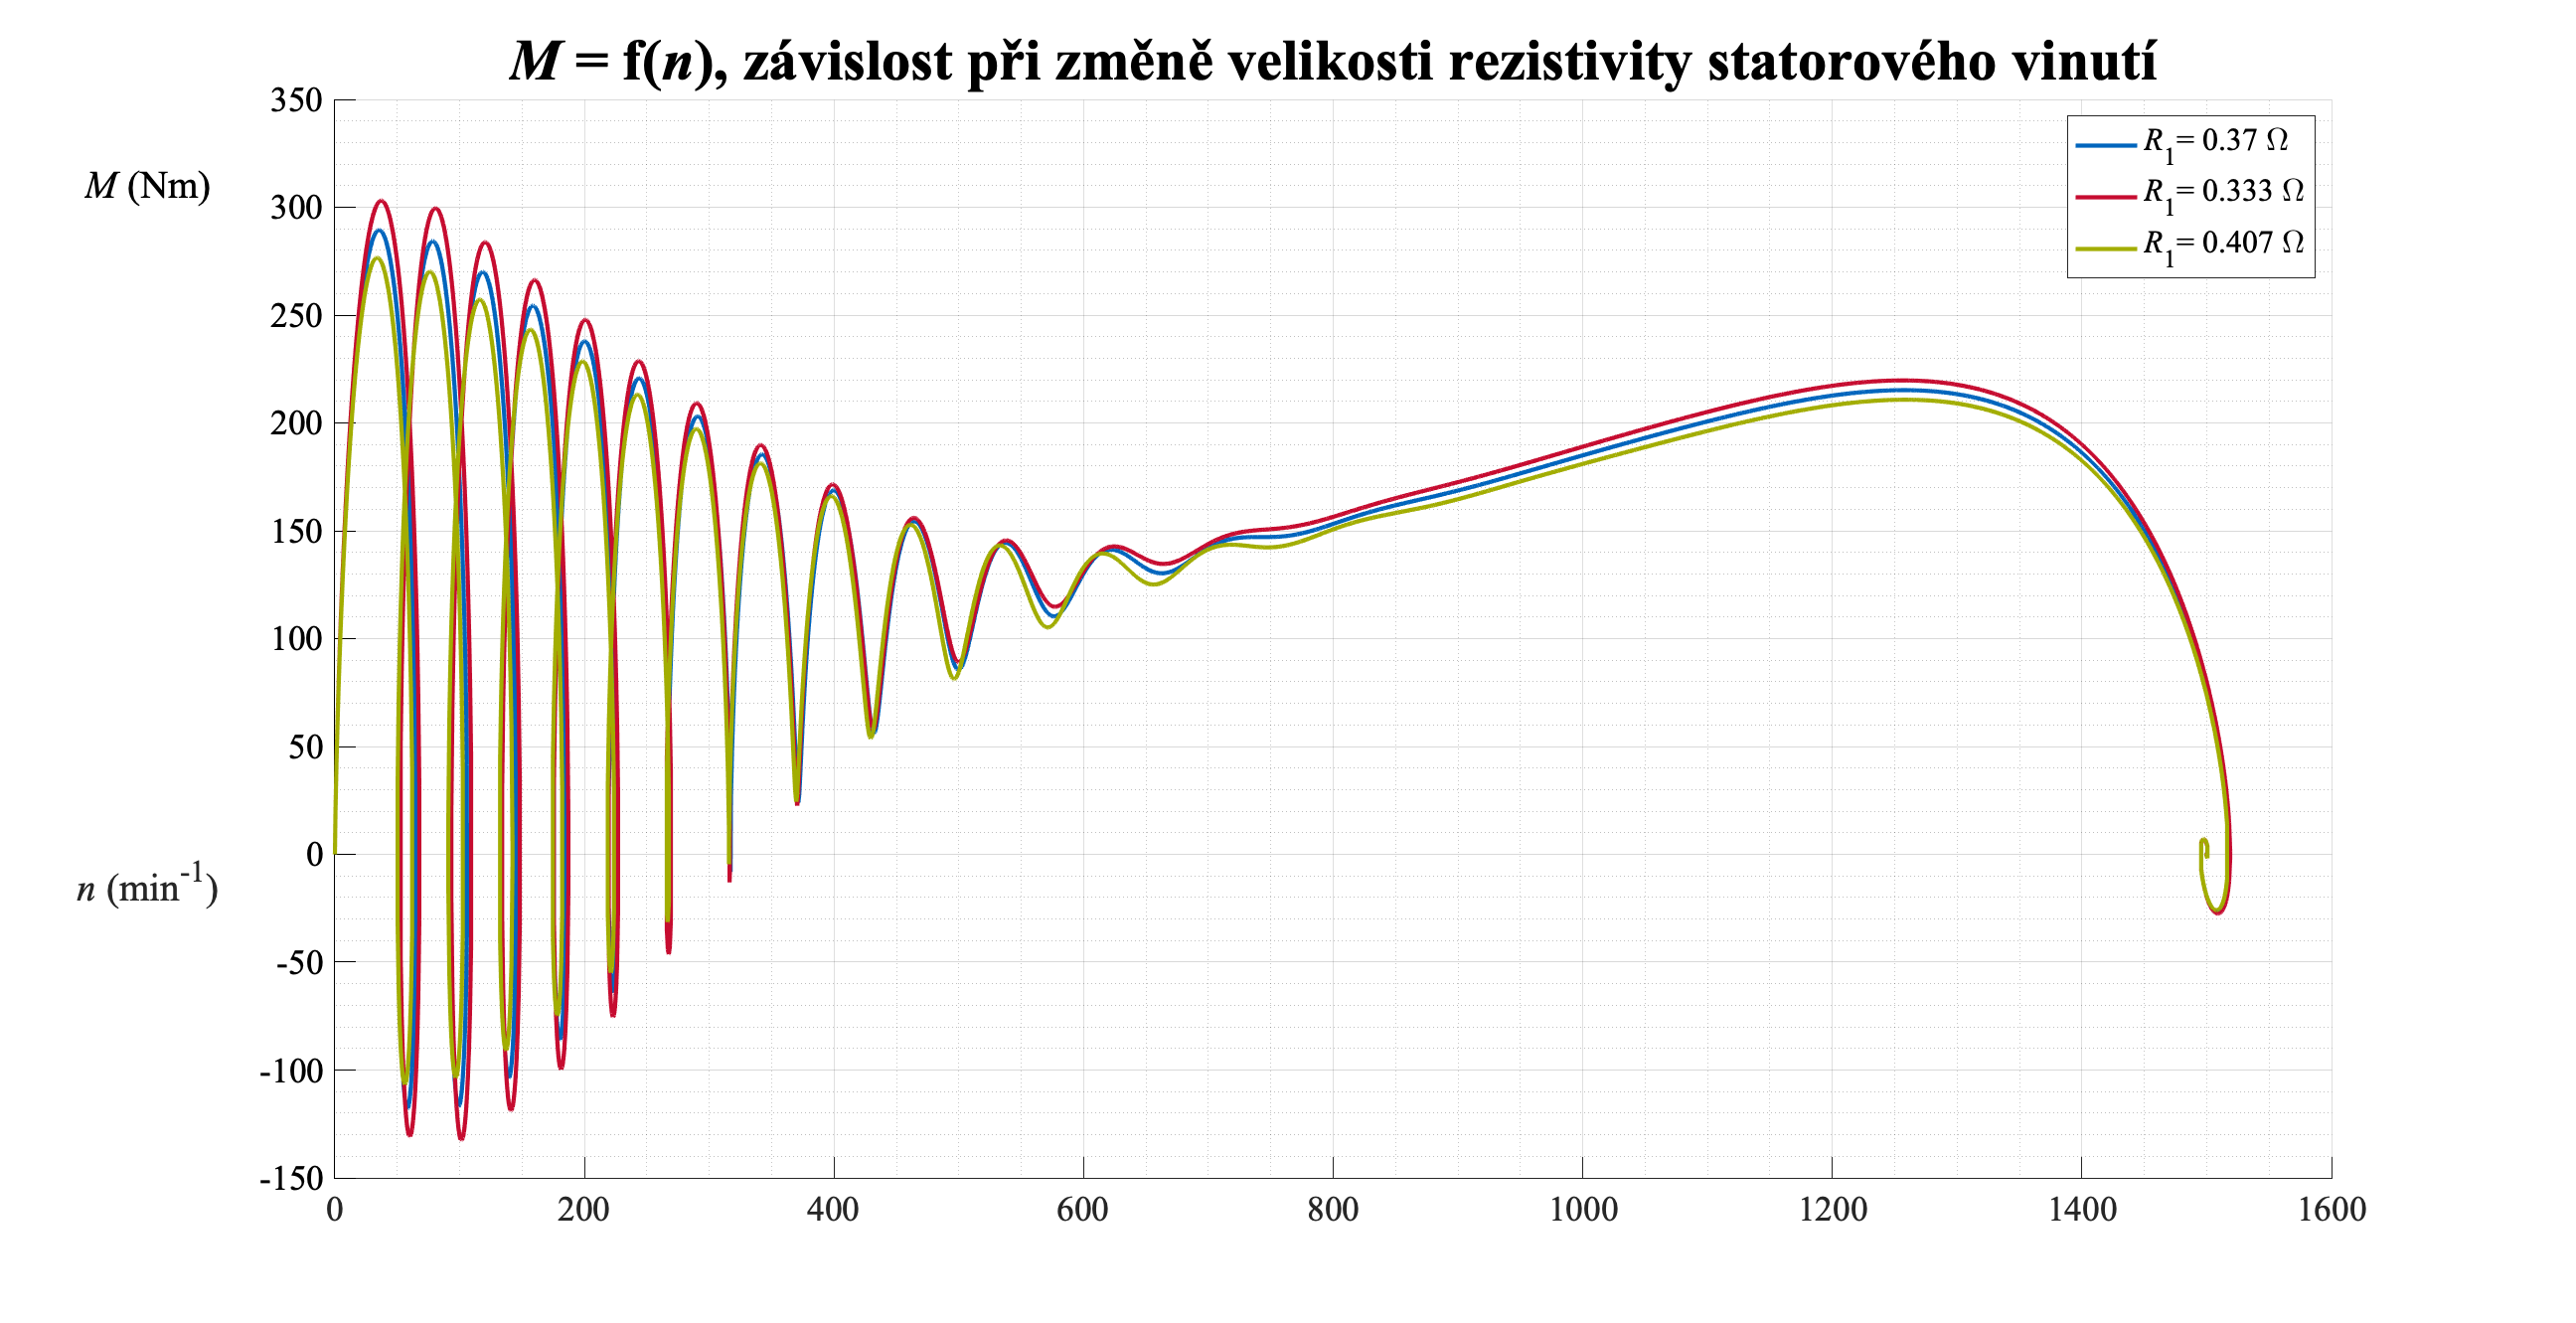
\includegraphics[width=1\textwidth]{src/png/mh_dyn_nGraphR1.png}
            \caption{Závislost elektromagnetického hnacího momentu \gls{symbol:m} na otáčkách stroje, vynesená při změně rezistivity statorového viutí o $\pm 10 \%$.}
            \label{fig:mh_dyn_nGraphR1}
        \end{figure}

\newpage

    \fbar
    \subsection{Změna magnetizační indukčnosti stroje}
        \begin{figure}[htbp!]
            \centering
            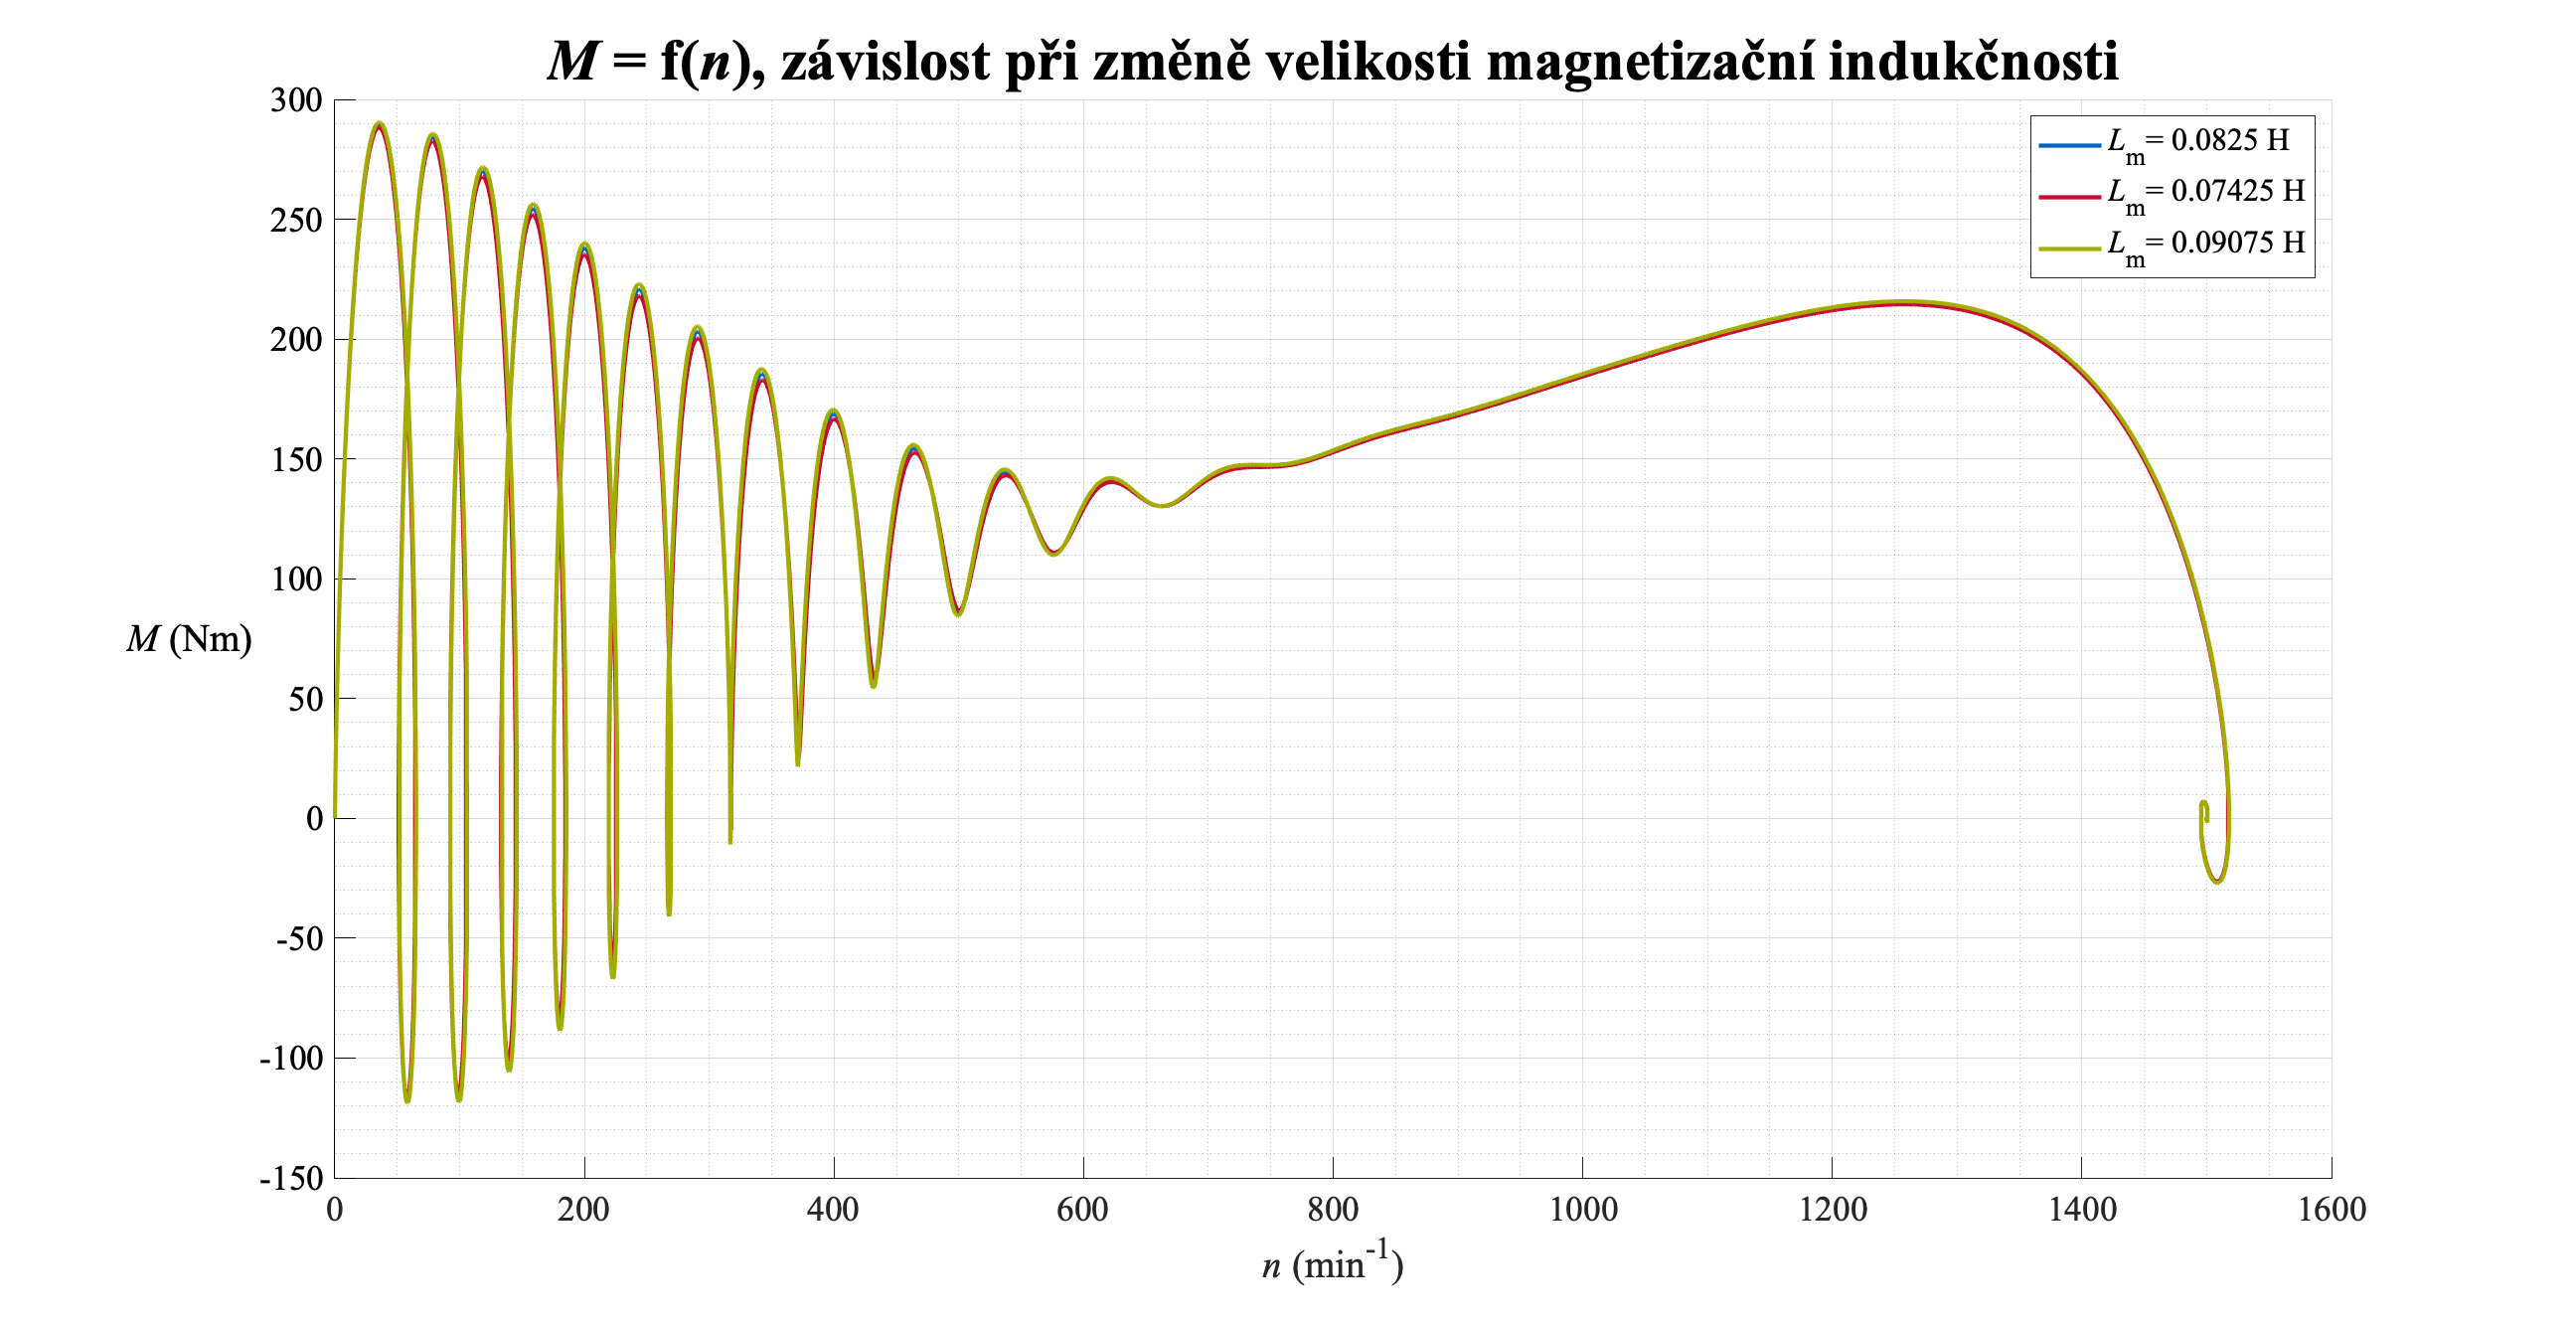
\includegraphics[width=1\textwidth]{src/png/mh_dyn_nGraphLm.png}
            \caption{Závislost elektromagnetického hnacího momentu \gls{symbol:m} na otáčkách stroje, vynesená při změně magnetizační indukčnosti o $\pm 10 \%$.}
            \label{fig:mh_dyn_nGraphLm}
        \end{figure}


    \fbar
    \subsection{Změna rozptylové indukčnosti statorového vinutí stroje}
        \begin{figure}[htbp!]
            \centering
            
\includegraphics[width=1\textwidth]{src/png/mh_dyn_nGraphL1sigma.png}
            \caption{Závislost elektromagnetického hnacího momentu \gls{symbol:m} na otáčkách stroje, vynesená při změně rozptylové indukčnosti statorového vinutí o $\pm 10 \%$.}
            \label{fig:mh_dyn_nGraphL1sigma}
        \end{figure}

    \newpage
    \fbar
    \subsection{Změna rozptylové indukčnosti rotorového vinutí stroje}
        \begin{figure}[htbp!]
            \centering
            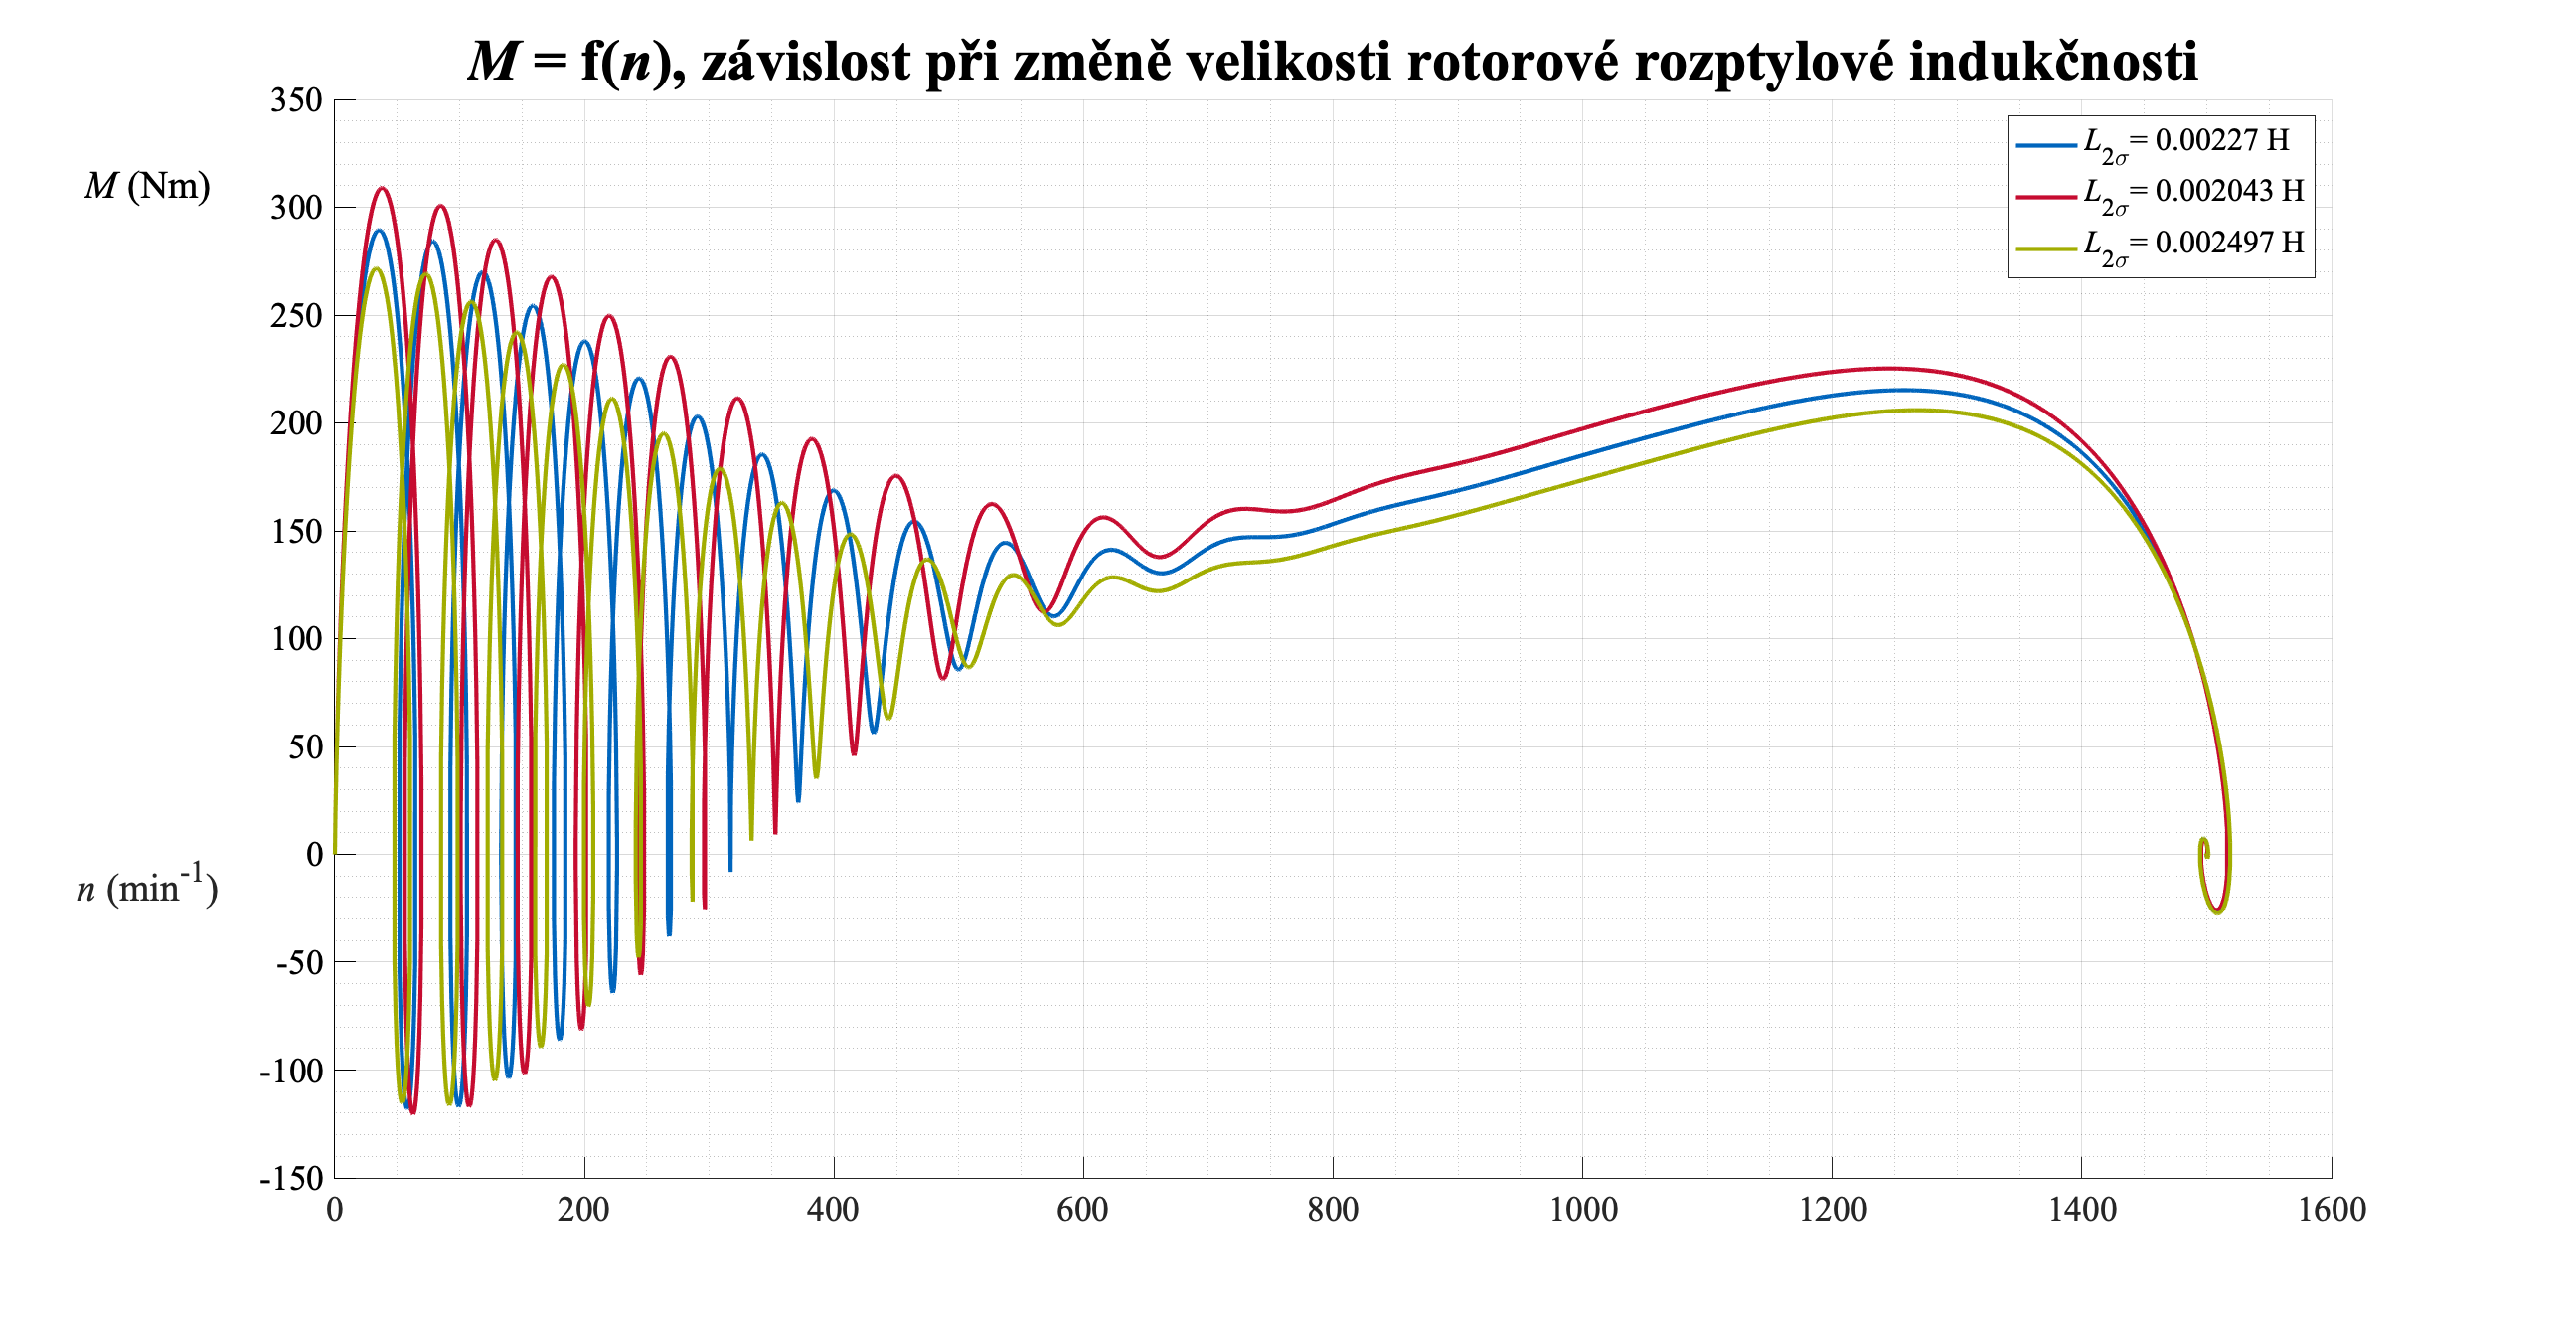
\includegraphics[width=1\textwidth]{src/png/mh_dyn_nGraphL2sigma.png}
            \caption{Závislost elektromagnetického hnacího momentu \gls{symbol:m} na otáčkách stroje, vynesená při změně rozptylové indukčnosti rotorového vinutí o $\pm 10 \%$.}
            \label{fig:mh_dyn_nGraphL2sigma}
        \end{figure}


%závěr
\newpage
\addcontentsline{toc}{section}{\numberline{}Zhodnocení} 
\section*{Zhodnocení}
Z představených průběhů závislosti elektromagnetického momentu stroje \gls{symbol:m} na otáčkách $n$ je možné vypozorovat, že největší vliv na změnu průběhu má změna rezistivity rotoru \gls{symbol:r2} a změna rozptylové indukčnosti statorového vinutí \gls{symbol:l1sigma} a rotoru \gls{symbol:l2sigma}.\par
Při zvýšení rezistivity rotoru dochází dle teorie k „pokládání“ charakteristiky a zvýšení záběrného momentu stroje. Proto jeden z možných způsobů rozběhu stroje s vinutou kotvou je rozběh se zvýšením rotorového odporu. Zvýšení rezistivity může být také zapříčeněno ohřevem stroje.\par
Změna velikosti rezistivity statorového vinutí se projevuje opačným způsobem, než změna rezistivity rotoru. Při snížení rezistivity vinutí dochází ke zvýšení velikosti elektromagnetického momentu stroje nad hodnotu, než která je pozorována při původní měřené hodnotě rezistivity. Naopak při zvýšení rezistivity vinutí dochází ke snížení vnitřního elektromagnetického momentu.\par
Zvýšení rozptylové indukčnosti statorového vinutí a rotoru se opět projevuje opačným způsobem, než změna rezistivity rotoru. Při snížení indukčnosti dochází ke zvýšení hodnoty elektromagnetického momentu při určitých otáčkách stroje. Při zvýšení rozptylové indukčnosti ke snížení momentu. Z teoretických předpokladů je zřejmé, že je vyžadována co nejmenší hodnota rozptylového magnetického toku, který se uzavírá cestami, které jsou odlišné od cesty hlavního magnetizačního toku. Simulace tento předpoklad potvrzuje.\par
Změna magnetizační indukčnosti \gls{symbol:lm} prakticky nemá vliv na představenou závislost elektromagnetického momentu.\par
Pozorované změny odpovídají teoretickým předpokladům o změně statické charakteristiky vnitřního elektromagnetického momentu stroje na otáčkách a je je tudíž možné aplikovat i na dynamickou závislost elektromagnetického momentu.

\flushbottom %vyčištění stránky

%konec závěru

\newpage
\setmonofont{Times New Roman}
\printbibliography[title={{Literatura}}]	
\nocite{*}
\setmonofont{CourierPrime-Regular}
\addcontentsline{toc}{section}{\numberline{}Literatura} %Added citations to TOC%
	\appendix
	\titleformat{\section}{\color{ctublue}\fontspec{Times New Roman}\fontsize{15}{15}\bfseries}{Appendix \thesection:}{2.1em}{}
	\begin{appendices}
	\section{Seznam symbolů a zkratek}

		\printglossary[type=abbreviationslist, style = myStyleAbbreviations]

		\fbar
		%\newpage
		\printglossary[type=symbolslist, style =  myStyleSymbols]

	\end{appendices}
\end{document}
